% \chapter{第四章	手写数字及写字人识别实验过程及其结果}
% \section{手写数字识别实验}
% \subsection{样本简介}

% 本论文的手写数字识别实验当中所用的样本分为两类,一类是训练样本集,另一类是测试样本集。
% 实验当中的训练样本集采用的是手写数字MNIST数据库。这个数据库当中包含训练集样本60000个样例和测试集样本10000个样例。MNIST数据库当中的数字样本已经全部大小归一化灰度化并且集中到同一个固定大小的图像当中。该数据库包括MST的SD-1和SD-3数据库,当中包含一系列的二级制的手写数字图像。其中SD-1的收集者来源是某高中的在校学生,而SD-3是由人口调查局员工收集的。则我们的训练样本集也就是MNIST当中的训练样本集有30000个样本来自SD-3,而另外30000个样本来自SD-1。这60000个训练样本分别来自约250个采集者。
% \subsection{Writer Depend类数字识别实验}
% \subsubsection{ABCvsA数字识别实验}
% 实验内容:以A写字人、B写字人和C写字人,合计3000个数字0到9的数字图像数据为训练样本集。A写字人的1000个数字0到9的数字图像数据为测试样本集。学习率为1,单次训练样本数为10个,共训练40次。若识别所得数字与给定的标签匹配,则视为正确;不匹配则视为错误。
% \begin{table}[htbp]
%     \centering
%     \caption{ABCvsA数字识别实验结果}
%     \label{tab:1}
%     \begin{tabular}{@{}cccc@{}}
%         \toprule
%         训练样本 & ABC & 样本个数    & 3000    \\ \midrule
%         测试样本 & A   & 样本个数    & 1000    \\
%         训练次数 & —   & 单次训练样本数 & 10      \\
%         学习率  & 1   & 正确率     & 99.50\% \\ \bottomrule
%     \end{tabular}
% \end{table}

% \subsubsection{ABCvsABC数字识别实验}
% 实验内容:以A写字人、B写字人和C写字人,合计3000个数字0到9的数字图像数据为总样本集。在总样本集当中随机抽取2400个为训练样本集,余下的600个为测试样本集。学习率为1,单次训练样本数为10个,共训练40次。若识别所得数字与给定的标签匹配,则视为正确;不匹配则视为错误。
% \begin{table}[htbp]
%     \centering
%     \caption{ABCvsABC数字识别实验结果}
%     \label{tab:2}
%     \begin{tabular}{@{}cccc@{}}
%         \toprule
%         训练样本 & ABC & 样本个数    & 2400    \\ \midrule
%         测试样本 & ABC & 样本个数    & 600     \\
%         训练次数 & 40  & 单次训练样本数 & 10      \\
%         学习率  & 1   & 正确率     & 92.00\% \\ \bottomrule
%     \end{tabular}
% \end{table}
% \subsection{Writer Depend类数字识别实验结果分析}

% 下面我们选取Writer Depend类数字识别实验当中的两个典型的例子ABCvsA数字识别实验以及MNIST\&ABCvsA数字识别实验的结果做详细分析。我们从ABCvsA数字识别实验中的训练样本集和测试样本集的手写数字图像样本集当中分别随机抽取一幅图像\ref{fig:complex}所示。

% \begin{figure}[htbp] % image examples & compare
%     \begin{subfigure}{0.5\textwidth}
%         \centering
%         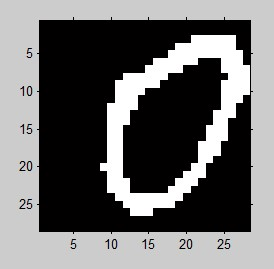
\includegraphics[height=6.54cm]{image/chap04/1.jpg}
%         \caption{实验训练集}
%         \label{fig:compare1}
%     \end{subfigure}
%     \begin{subfigure}{0.5\textwidth}
%         \centering
%         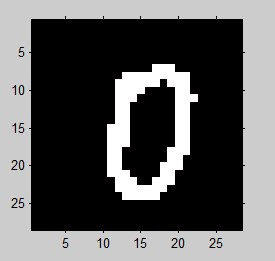
\includegraphics[height=6.54cm]{image/chap04/2.jpg}
%         \caption{实验测试集}
%         \label{fig:compare2}
%     \end{subfigure}
%     \caption{ABCvsA数字识别实验集}
%     \label{fig:complex}
% \end{figure}

% 下面我们对上述的训练集和测试集进行40次学习率为2,单次训练样本为10的迭代,得到错误率为0.50\%,而其中每次训练时的误差值组成的历史误差值画图分析如下:
% ……
% \subsection{Writer Independ类数字识别实验}
% 实验内容:以MNIST数据库为训练样本集,共计60000个训练样本。以A写字人合计1000个数字0到9的数字图像数据为测试样本集写字人识别实验
% ……
% \subsection{样本简介}
% ……
% \subsection{两位写字人识别实验}
% \subsubsection{单个数字的写字人识别实验}
% 实验内容:以A写字人,合计800个数字5的数字图像数据加上B写字人,合计800个数字5的数字图像数据,共计1600个样本为总样本集。随机选取其中的1200个样本为训练样本集,其余的400个样本为测试样本集。学习率为2,单次训练样本数为10个,共训练30次。若识别所得写字人与给定的标签匹配,则视为正确;不匹配则视为错误。
% \begin{table}[]
%     \centering
%     \caption{单个数字写字人识别实验结果}
%     \label{tab:3}
%     \begin{tabular}{@{}cccc@{}}
%         \toprule
%         训练样本 & A5\&B5 & 样本个数    & 1200    \\ \midrule
%         测试样本 & A5\&B5 & 样本个数    & 400     \\
%         训练次数 & 30     & 单次训练样本数 & 10      \\
%         学习率  & 2      & 正确率     & 99.75\% \\ \bottomrule
%     \end{tabular}
% \end{table}
% \subsubsection{单个数字的写字人识别实验结果分析}

% ……
% \section{本章小结}

% ……。

\chapter{数值实验}

\section{汽车的动态模型}

在本节中,我们通过一个真实场景示例展示卡尔曼滤波器的强大能力及其捕捉马尔可夫过程行为的效果。我们考虑一个汽车的动态模型,该模型在二维坐标系中模拟汽车的运动,并跟踪其位置与速度。转移矩阵 \(\mathbf{A}\) 定义如下:

\begin{align}
    \begin{pmatrix}
        x_k^{(1)} \\
        x_k^{(2)} \\
        x_k^{(3)} \\
        x_k^{(4)}
    \end{pmatrix} = \underbrace{
    \begin{pmatrix}
    1 & 0 & \Delta t & 0 \\
    0 & 1 & 0 & \Delta t \\
    0 & 0 & 1 & 0 \\
    0 & 0 & 0 & 1
    \end{pmatrix}}_{\mathbf{A}}
    \begin{pmatrix}
    x_{k-1}^{(1)} \\
    x_{k-1}^{(2)} \\
    x_{k-1}^{(3)} \\
    x_{k-1}^{(4)}
    \end{pmatrix}
    +
    \mathbf{q}_{k-1}, \label{eq: exp car A}
\end{align}

其中 \(\mathbf{q}_{k-1}\) 是一个离散时间高斯噪声过程,其均值为零,协方差矩阵 \(\mathbf{Q}\) 定义为:

\begin{align}
    \mathbf{Q} = 
    \begin{pmatrix}
    \frac{q_{1}^c \Delta t^3}{3} & 0 & \frac{q_{1}^c \Delta t^2}{2} & 0 \\
    0 & \frac{q_{2}^c \Delta t^3}{3} & 0 & \frac{q_{2}^c \Delta t^2}{2} \\
    \frac{q_{1}^c \Delta t^2}{2} & 0 & q_{1}^c \Delta t & 0 \\
    0 & \frac{q_{2}^c \Delta t^2}{2} & 0 & q_{2}^c \Delta t
    \end{pmatrix}.
\end{align}

该动态系统的线性高斯状态空间模型(LGSSM)完整形式为:

\begin{align}
    \mathbf{x}_k &= \mathbf{A}_{k-1} \mathbf{x}_{k-1} + \mathbf{q}_{k-1}, \\
    \mathbf{y}_k &= \mathbf{H}_k \mathbf{x}_{k} + \mathbf{r}_{k},
\end{align}

其中模型参数设置如下:
\begin{itemize}
    \item \(\mathbf{A}_{k-1}\) 按照式~\eqref{eq: exp car A} 定义,
    \item \(\mathbf{H}_k = \mathbf{I}_4\),
    \item \(\mathbf{r}_k \sim \mathcal{N}(\mathbf{0}, \sigma_\mathbf{r}^2 \mathbf{I}_4)\),其中 \(\sigma_\mathbf{r} = 0.1\),
    \item \(\mathbf{x}_0 \sim \mathcal{N}(\mathbf{m}_0, \mathbf{P}_0)\),其中 \(\mathbf{m}_0 = \mathbf{0}\),\(\mathbf{P}_0 = \sigma_\mathbf{P}^2 \mathbf{I}_4\),\(\sigma_\mathbf{P} = 0.1\)。
\end{itemize}

该模型表示的是匀速运动,其中状态向量的前两个分量对应位置,后两个分量对应速度。卡尔曼滤波器与平滑器为估计观测数据背后的潜在状态变量提供了闭式解法。

\begin{figure}
    \centering
    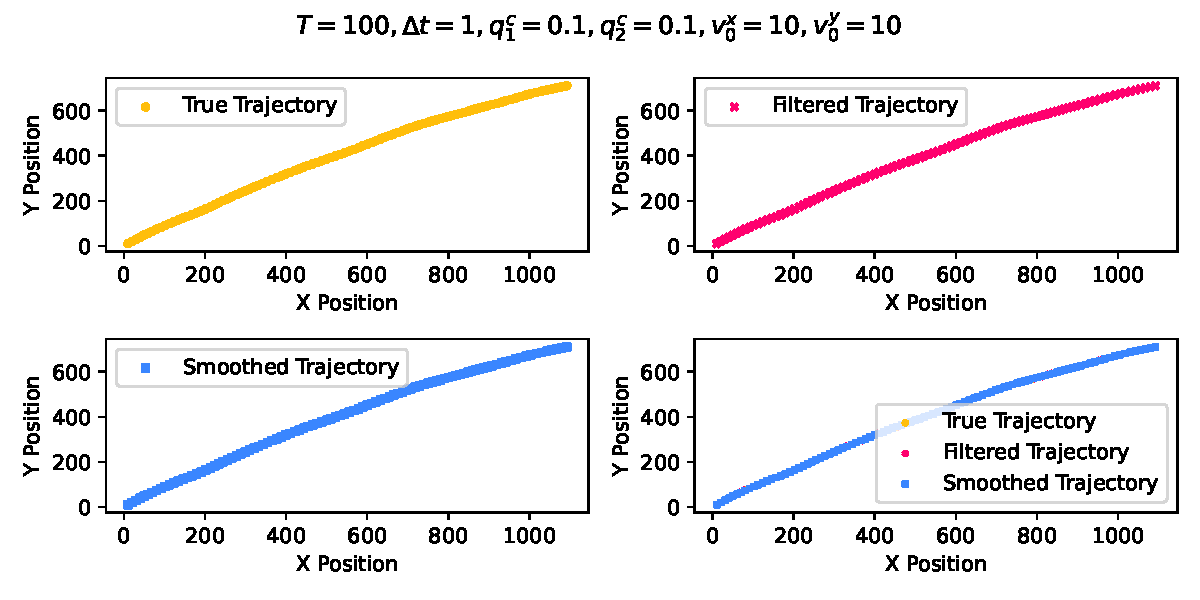
\includegraphics[width=0.95\linewidth]{fig/estimated_car_trajectory.pdf}
    \caption{观测轨迹与使用卡尔曼滤波器和平滑器估计得到的轨迹。}
    \label{fig: exp car trajectory}
\end{figure}

图~\ref{fig: exp car trajectory} 展示了实验结果,绘制了使用卡尔曼滤波器和平滑器所估计的轨迹。该图直观展示了这些方法在准确估计潜在状态变量方面的有效性。

我们还使用经典的期望最大化(EM)算法对该汽车模型的参数进行估计。EM 算法是状态空间模型中广泛应用的参数估计方法,我们将在该示例中评估其性能。

\begin{table}[tb]
\centering
\caption{汽车模型的 EM 算法结果。基线负对数似然为 \(\mathcal{L}_T({\boldsymbol{\theta}}) = -261.989\)。}
\label{tab: exp car EM results}
\begin{tabular}{lll}
\toprule
\textbf{待估参数} & \textbf{\(\mathcal{L}_T(\widehat{\boldsymbol{\theta}})\)} & \textbf{\(\| \widehat{\boldsymbol{\theta}} - \boldsymbol{\theta} \|_F\)} \\
\midrule
\(\mathbf{A}\) & -273.250 & 0.248 \\
\(\mathbf{Q}\) & -247.424 & 0.308 \\
\(\mathbf{H}\) & -169.839 & 0.642 \\
\bottomrule
\end{tabular}
\end{table}

表~\ref{tab: exp car EM results} 总结了使用 EM 算法对参数 \(\mathbf{A}\)、\(\mathbf{Q}\) 和 \(\mathbf{H}\) 的估计结果。表中列出了每个估计参数对应的负对数似然值 \(\mathcal{L}_T(\widehat{\boldsymbol{\theta}})\) 以及与真实参数之间的 Frobenius 范数 \(\| \widehat{\boldsymbol{\theta}} - \boldsymbol{\theta} \|_F\)。

\begin{figure}[tb]
    \centering
    \begin{subfigure}[b]{0.95\textwidth}
        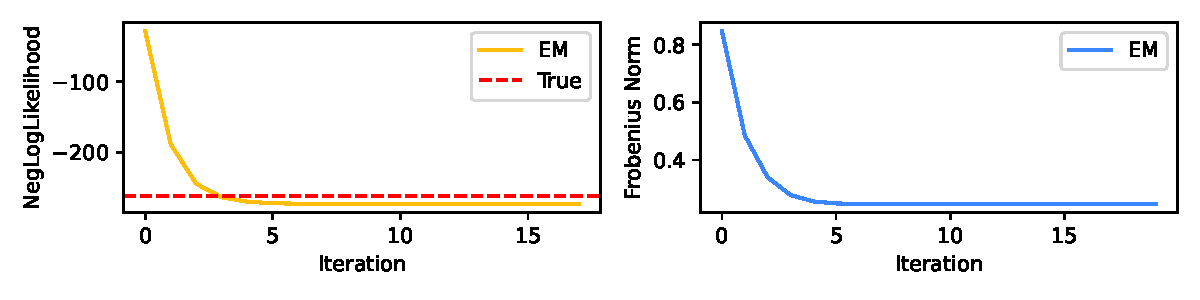
\includegraphics[width=\textwidth]{fig/A_neg_log_likelihood_fnorm.pdf}
        \caption{\(\mathbf{A}\) 的负对数似然与 Frobenius 范数变化。}
        \label{fig:subfig1}
    \end{subfigure}
    
    \begin{subfigure}[b]{0.95\textwidth}
        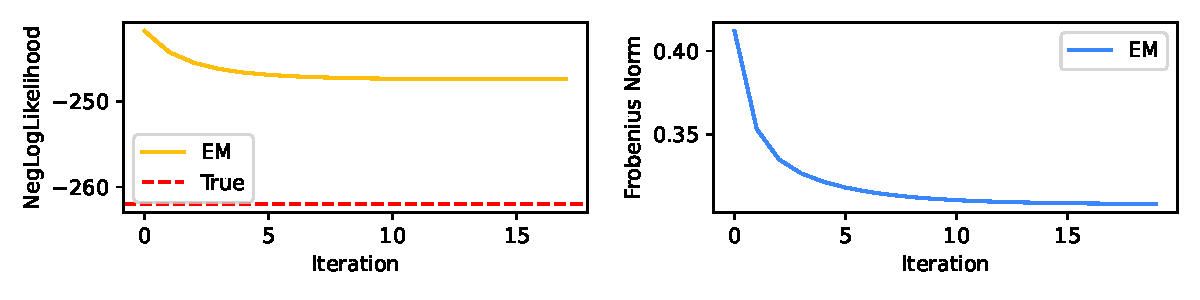
\includegraphics[width=\textwidth]{fig/Q_neg_log_likelihood_fnorm.pdf}
        \caption{\(\mathbf{Q}\) 的负对数似然与 Frobenius 范数变化。}
        \label{fig:subfig2}
    \end{subfigure}

    \begin{subfigure}[b]{0.95\textwidth}
    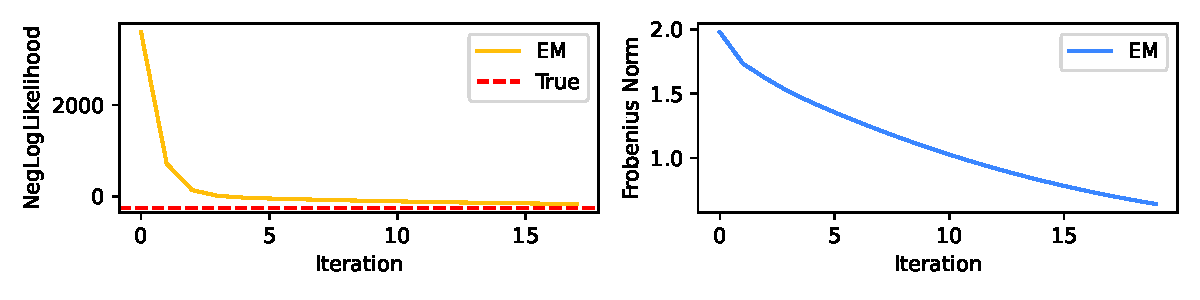
\includegraphics[width=\textwidth]{fig/H_neg_log_likelihood_fnorm.pdf}
    \caption{\(\mathbf{H}\) 的负对数似然与 Frobenius 范数变化。}
    \end{subfigure}
    \caption{EM 算法在估计 \(\mathbf{A}\)、\(\mathbf{Q}\) 和 \(\mathbf{H}\) 时的性能可视化结果。}
    \label{fig: exp car EM visualization}
\end{figure}

\begin{figure}[tb]
    \centering
    \begin{subfigure}[b]{0.85\textwidth}
        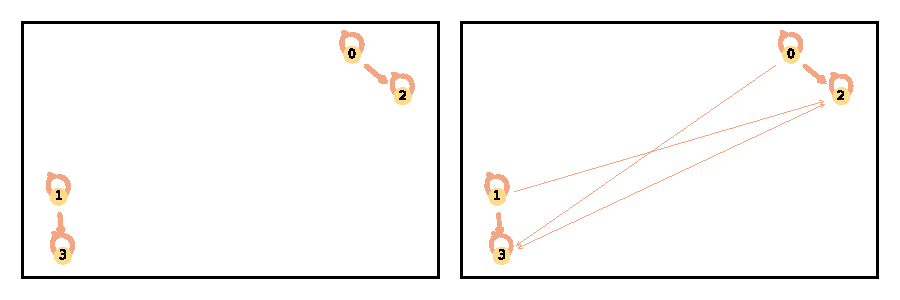
\includegraphics[width=\textwidth]{fig/A_graphs_for_true_and_EM.pdf}
        \caption{\(\mathbf{A}\) 的图结构表示:左为真实值,右为估计值。}
        \label{fig:subfig1}
    \end{subfigure}
    
    \begin{subfigure}[b]{0.85\textwidth}
        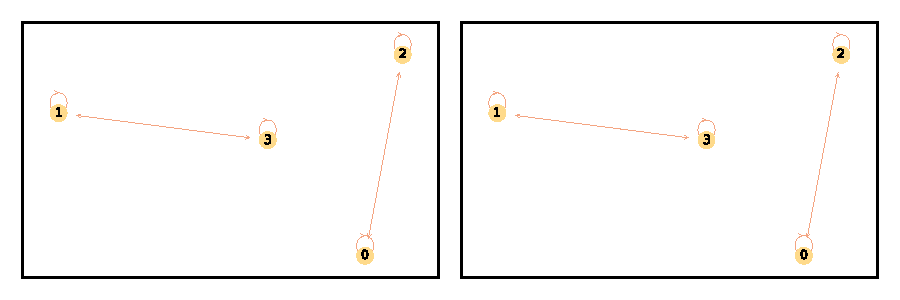
\includegraphics[width=\textwidth]{fig/Q_graphs_for_true_and_EM.pdf}
        \caption{\(\mathbf{Q}\) 的图结构表示:左为真实值,右为估计值。}
        \label{fig:subfig2}
    \end{subfigure}

    \begin{subfigure}[b]{0.85\textwidth}
    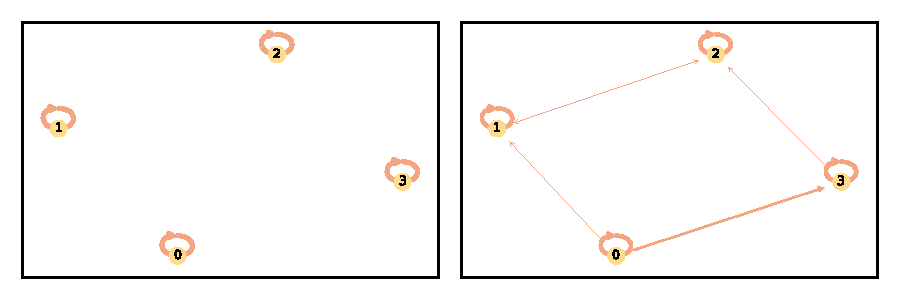
\includegraphics[width=\textwidth]{fig/H_graphs_for_true_and_EM.pdf}
    \caption{\(\mathbf{H}\) 的图结构表示:左为真实值,右为估计值。}
    \end{subfigure}
    \caption{真实参数与估计参数 \(\mathbf{A}\)、\(\mathbf{Q}\)、\(\mathbf{H}\) 的图形对比。}
    \label{fig: exp car graph comparison}
\end{figure}

为进一步直观展示参数估计过程,图~\ref{fig: exp car EM visualization} 展示了 EM 迭代中每个参数对应的负对数似然与 Frobenius 范数的变化趋势。此外,图~\ref{fig: exp car graph comparison} 给出了各参数的图结构对比图,分别显示了真实值与估计结果之间的差异。
    
\section{不同图结构下的正则化分析}

在本节中,我们介绍实验中使用的不同图结构的数学特性。这些结构在 GraphEM 算法中起到了定义转移矩阵正则化先验的关键作用。下文将对每种图类型进行详细分析,并说明其生成所采用的具体参数。

\paragraph*{分块对角结构(Blockwise-Diagonal)}
分块对角矩阵是一类特殊的稀疏矩阵,其非零元素局限于对角线上的若干块中。数学形式如下:
\[
\mathbf{A} = \begin{pmatrix}
\mathbf{A}_1 & \mathbf{0} & \cdots & \mathbf{0} \\
\mathbf{0} & \mathbf{A}_2 & \cdots & \mathbf{0} \\
\vdots & \vdots & \ddots & \vdots \\
\mathbf{0} & \mathbf{0} & \cdots & \mathbf{A}_k
\end{pmatrix},
\]
其中 \(\mathbf{A}_i\) 是子矩阵,\(\mathbf{0}\) 表示相应维度的零矩阵。该结构常用于建模解耦或弱耦合的子系统。

\paragraph*{小世界图(Small-World)}
小世界图具有较高的聚类系数与较短的平均路径长度。在实验中,我们使用 Watts-Strogatz 模型生成小世界图,设节点数 \(n = 16\),每个节点连接 \(k = 4\) 个最近邻节点,重连概率为 \(p = 0.3\)。小世界图的邻接矩阵 \(\mathbf{A}\) 通常具有局部连接与少量远程连接的混合特性,实现稀疏性与连通性的平衡。

\paragraph*{无标度图(Scale-Free)}
无标度图的节点度分布满足幂律形式:\(P(k) \sim k^{-\gamma}\),其中 \(k\) 是节点度,\(\gamma\) 是常数。我们使用 Barabási-Albert 模型生成无标度图,设 \(n = 16\),每步增加 \(m = 2\) 条边。该图的邻接矩阵 \(\mathbf{A}\) 高度稀疏,仅有少数枢纽节点具有较高的度数。

\paragraph*{二部图(Bipartite)}
二部图是一类可将顶点划分为两个不相交集合 \(U\) 与 \(V\) 的图,其中每条边仅连接 \(U\) 与 \(V\) 中的节点。实验中,我们生成一个完全二部图,节点数 \(n = 16\),两个子集分别为 \(n_1 = \lfloor n/2 \rfloor\)、\(n_2 = \lfloor n/2 \rfloor\)。其邻接矩阵形式如下:
\[
\mathbf{A} = \begin{pmatrix}
\mathbf{0} & \mathbf{B} \\
\mathbf{B}^\top & \mathbf{0}
\end{pmatrix},
\]
其中 \(\mathbf{B}\) 是表示两个集合间连接关系的矩阵。该结构适用于建模两个不同实体间的关联关系。

\paragraph*{环图(Cycle)}
环图由一个封闭的循环组成,每个节点恰好与两个其他节点相连。我们生成节点数为 \(n = 16\) 的环图。其邻接矩阵为循环矩阵(circulant matrix):
\[
\mathbf{A} = \begin{pmatrix}
0 & 1 & 0 & \cdots & 1 \\
1 & 0 & 1 & \cdots & 0 \\
0 & 1 & 0 & \cdots & 0 \\
\vdots & \vdots & \vdots & \ddots & \vdots \\
1 & 0 & 0 & \cdots & 0
\end{pmatrix}.
\]
环图常用于建模周期性或循环性结构。

\paragraph*{星型图(Star)}
星型图由一个中心节点与所有其他节点连接而成,其他节点之间没有连接。实验中,我们生成 \(n = 16\) 节点的星型图。其邻接矩阵为:
\[
\mathbf{A} = \begin{pmatrix}
0 & 1 & 1 & \cdots & 1 \\
1 & 0 & 0 & \cdots & 0 \\
1 & 0 & 0 & \cdots & 0 \\
\vdots & \vdots & \vdots & \ddots & \vdots \\
1 & 0 & 0 & \cdots & 0
\end{pmatrix}.
\]
星型图适用于建模中心化系统或星状网络结构(hub-and-spoke)。

\begin{table}[tb]
\centering
\caption{不同图结构在各类正则方法下的实验结果。每种图类型中加粗的数值表示最佳结果。}
\label{tab: prior results for block-diag}
\begin{tabular}{llll}
\toprule
\textbf{图类型} & \textbf{方法} & \textbf{\(\mathcal{L}_T(\widehat{\mathbf{A}})\)} & \textbf{\(\| \widehat{\mathbf{A}} - \mathbf{A} \|_F\)} \\
\midrule
分块对角 & EM & -21288.702 & 0.611 \\
 & GraphEM Laplace & -21262.253 & 0.575 \\
 & GraphEM Gaussian & -21287.225 & 0.608 \\
 & GraphEM Laplace+Gaussian & -21244.464 & \textbf{0.566} \\
小世界 & EM & -2237.305 & 2.489 \\
 & GraphEM Laplace & -2195.235 & 2.181 \\
 & GraphEM Gaussian & -2235.439 & 2.424 \\
 & GraphEM Laplace+Gaussian & -2193.343 & \textbf{2.140} \\
无标度 & EM & -2234.821 & 2.176 \\
 & GraphEM Laplace & -2197.950 & 2.005 \\
 & GraphEM Gaussian & -2233.167 & 2.138 \\
 & GraphEM Laplace+Gaussian & -2195.138 & \textbf{1.974} \\
二部图 & EM & -2228.962 & 2.366 \\
 & GraphEM Laplace & -2187.252 & 2.170 \\
 & GraphEM Gaussian & -2227.116 & 2.310 \\
 & GraphEM Laplace+Gaussian & -2185.598 & \textbf{2.127} \\
环图 & EM & -2279.460 & 2.257 \\
 & GraphEM Laplace & -2244.706 & 2.022 \\
 & GraphEM Gaussian & -2277.679 & 2.206 \\
 & GraphEM Laplace+Gaussian & -2243.051 & \textbf{1.984} \\
星型图 & EM & -2287.181 & 2.517 \\
 & GraphEM Laplace & -2253.640 & 2.240 \\
 & GraphEM Gaussian & -2285.723 & 2.456 \\
 & GraphEM Laplace+Gaussian & -2252.407 & \textbf{2.196} \\
\bottomrule
\end{tabular}
\end{table}

表~\ref{tab: prior results for block-diag} 总结了 EM 算法及其 GraphEM 变体(包括 Laplace、Gaussian 和 Laplace+Gaussian 正则化)在不同图结构上的性能表现,图类型包括分块对角、小世界、无标度、二部图、环图和星型图。表中报告了每种方法在每种图类型下的负对数似然 \(\mathcal{L}_T(\widehat{\mathbf{A}})\) 以及 Frobenius 范数 \(\| \widehat{\mathbf{A}} - \mathbf{A} \|_F\)。

从表中可以看出,GraphEM 的各类变体在 Frobenius 范数方面均优于标准 EM 算法。具体而言:
\begin{itemize}
    \item \textit{GraphEM Laplace+Gaussian} 方法在所有图类型中均表现最佳,取得了最小的 Frobenius 范数。这表明将 Laplace 与 Gaussian 先验结合能够提供更稳健的正则化框架。
    \item \textit{GraphEM Laplace} 方法相较标准 EM 同样具有显著提升,尤其在降低 Frobenius 范数方面效果明显,说明稀疏性正则化在刻画图结构方面是有效的。
    \item \textit{GraphEM Gaussian} 方法相比标准 EM 稍有提升,但整体效果不如 Laplace 及 Laplace \\ 
    + Gaussian 变体,进一步强调了诱导稀疏性的先验在图结构正则化中的重要性。
\end{itemize}

\begin{figure}[tb]
    \centering
    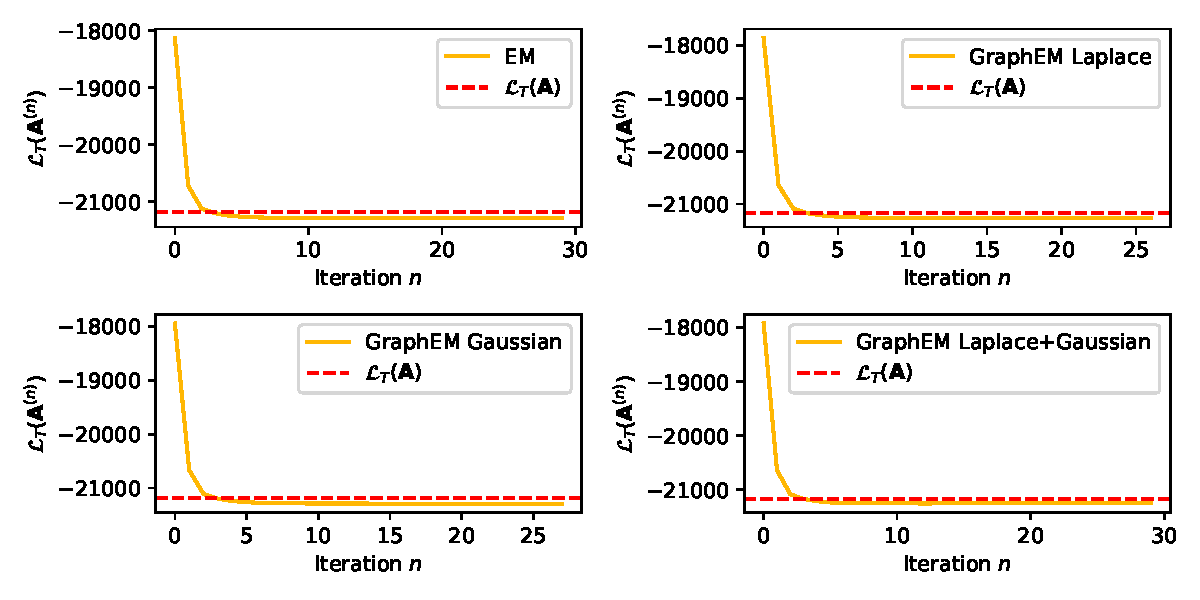
\includegraphics[width=0.85\linewidth]{fig/block diagonal/neg_log_likelihood.pdf}
    \caption{不同正则化方法下,分块对角图的负对数似然收敛曲线。}
    \label{fig: neg log likelihood}
\end{figure}

图~\ref{fig: neg log likelihood} 展示了分块对角图在不同正则方法下的负对数似然收敛情况。从图中可以看出,所有 EM 系列方法的收敛值均低于真实参数对应的负对数似然值,进一步验证了其估计效果的有效性。

\begin{figure}[tb]
    \centering
    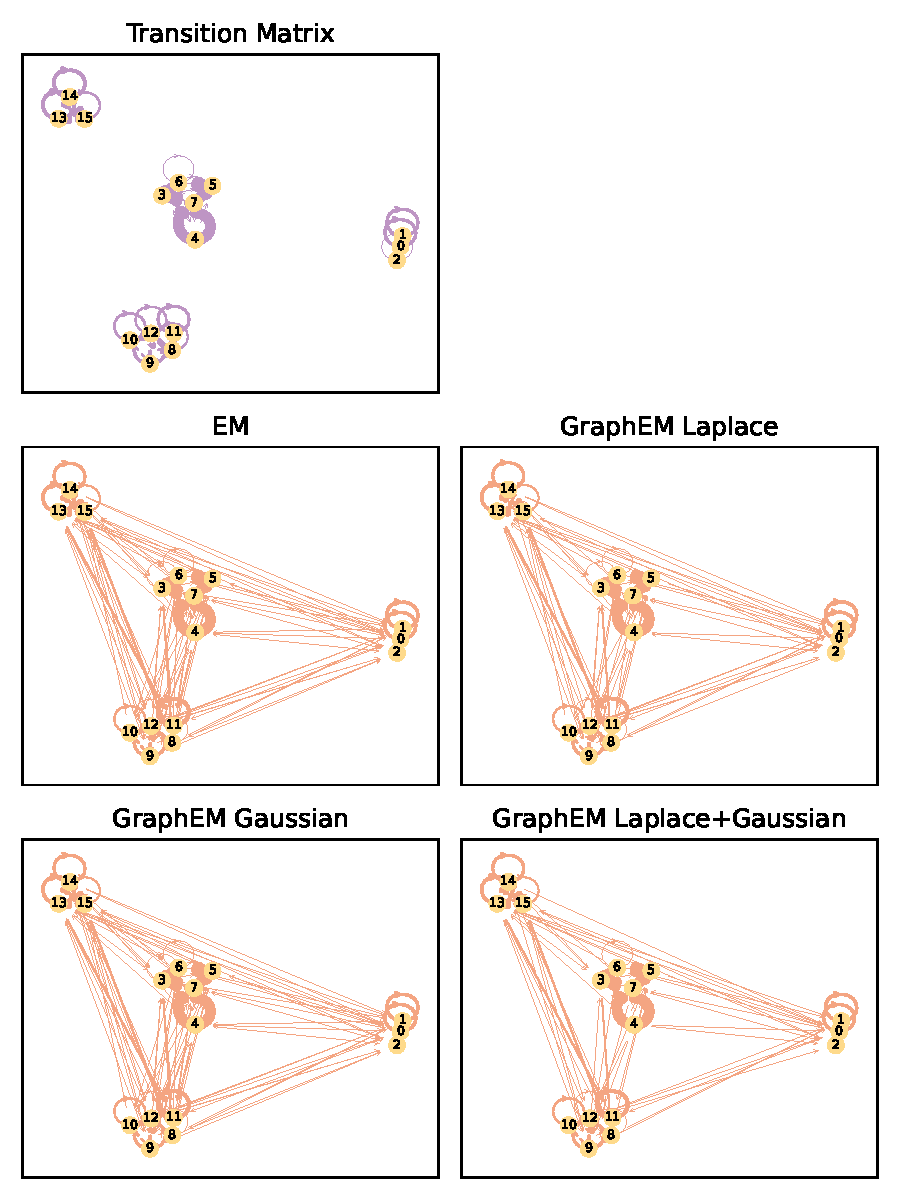
\includegraphics[width=0.75\linewidth]{fig/block diagonal/graphs_for_true_and_EM.pdf}
    \caption{分块对角图的真实转移矩阵与估计矩阵对比图。}
    \label{fig: graph comparison}
\end{figure}

为了进行更细致的对比,图~\ref{fig: graph comparison} 可视化展示了分块对角图的真实转移矩阵与估计转移矩阵。结果显示,GraphEM 的 Laplace 与 Laplace+Gaussian 方法所得估计最接近真实值,伪影更少,且更好地保留了块对角结构。

实验结果表明,将先验知识以正则化方式融入 EM 算法是有效的。具体而言:
\begin{itemize}
    \item \textit{Laplace 先验} 在促进稀疏性方面尤其有效,这对捕捉小世界图与无标度图等图结构至关重要。
    \item \textit{Gaussian 先验} 提供了更平滑的估计,但在保持稀疏性方面较弱,因此更适用于如二部图和环图这类相对稠密的结构。
    \item \textit{Laplace+Gaussian 先验} 综合了两种先验的优势,在所有图类型中表现最佳。这表明混合正则策略在图结构参数估计中具有高度通用性和效果。
\end{itemize}

这些发现突显了 GraphEM 在多种图结构上的优越性能。与标准 EM 算法相比,GraphEM 不仅保持了相当的收敛速度,而且在估计精度上有显著提升,进一步验证了其有效性。值得注意的是,在所有图类型中,在 Laplace 先验基础上引入 Gaussian 正则项的做法始终能进一步提升表现。这一现象可有两种解释:(1)稀疏性仍是这些图结构中的主导特征;或(2)算法对具体图类型具有一定鲁棒性。在这两种情形下,Gaussian 正则所引入的稳定性都能带来性能提升。

此外,我们还观察到,在 GraphEM 中将 Laplace 与 Gaussian 先验结合后,能够“无折中”地叠加两者的优点,而不会引入额外的优化计算开销。这一结果尤其具有前景意义,表明 GraphEM 的迭代优化框架可以无缝整合多种正则项。这一发现为未来研究开辟了新方向,即通过累积不同类型的正则项,在不增加计算复杂度的前提下迭代逼近最优解。
